\subsection{The data acquisition system }
\label{sec:DAQ}

%%%%%%%%%%%%%%%%%%%%%%%%%%%%%%%%%%%%%%%%%%%%%%%%%%%%%%%%%%%%%%%%%%%%%%%%%%%%%%%%%%%%
%by MMdevi. Last modified July 2, 2017.
%%%%%%%%%%%%%%%%%%%%%%%%%%%%%%%%%%%%%%%%%%%%%%%%%%%%%%%%%%%%%%%%%%%%%%%%%%%%%%%%%%%%


The DAQ system is heterogeneous using both 
NIM and VME electronic modules. The data readout is being carried out through a PCIe card \footnote{CAEN A3818 PCIe}  connected via an optical link to a VME controller\footnote{CAEN V2718 VME controller}. A schematic layout of the DAQ system is shown in Fig.~{\ref{Fig:DAQscheme}}. 

The PMTs are ramped up to their individual working voltage (corresponding to a gain of $2\times10^6$) using VME high voltage distributor module\footnote{iseg VDS18130p : 
24 independent channels positive polarity voltage distributer}. The raw pulses from the PMTs are amplified and shaped using 
two PMT preamplifiers\footnote{Phillips 776. 16 independent and direct-coupled amplifiers channels}. The preamplifier operates 
from DC to 275 MHz and produces two identical 50 $\Omega$ non inverting outputs with voltage gains of 10 for each PMT channel. One 
of the outputs is converted into a digital signal by an ADC\footnote{CAEN ADC V1742: switched capacitor digitizer}, and the other to 
binary signals using two discriminators\footnote{CAEN V895 16 channel leading edge discriminator}.

%%%%%%%%%%%%%%%%%%%%%%%%%%%%%%%%%%%%%%%%%%%%%%%%%%%%%%%%%%%%%%%%%%%%%%%%%%
\begin{figure}[h]
   \centering
   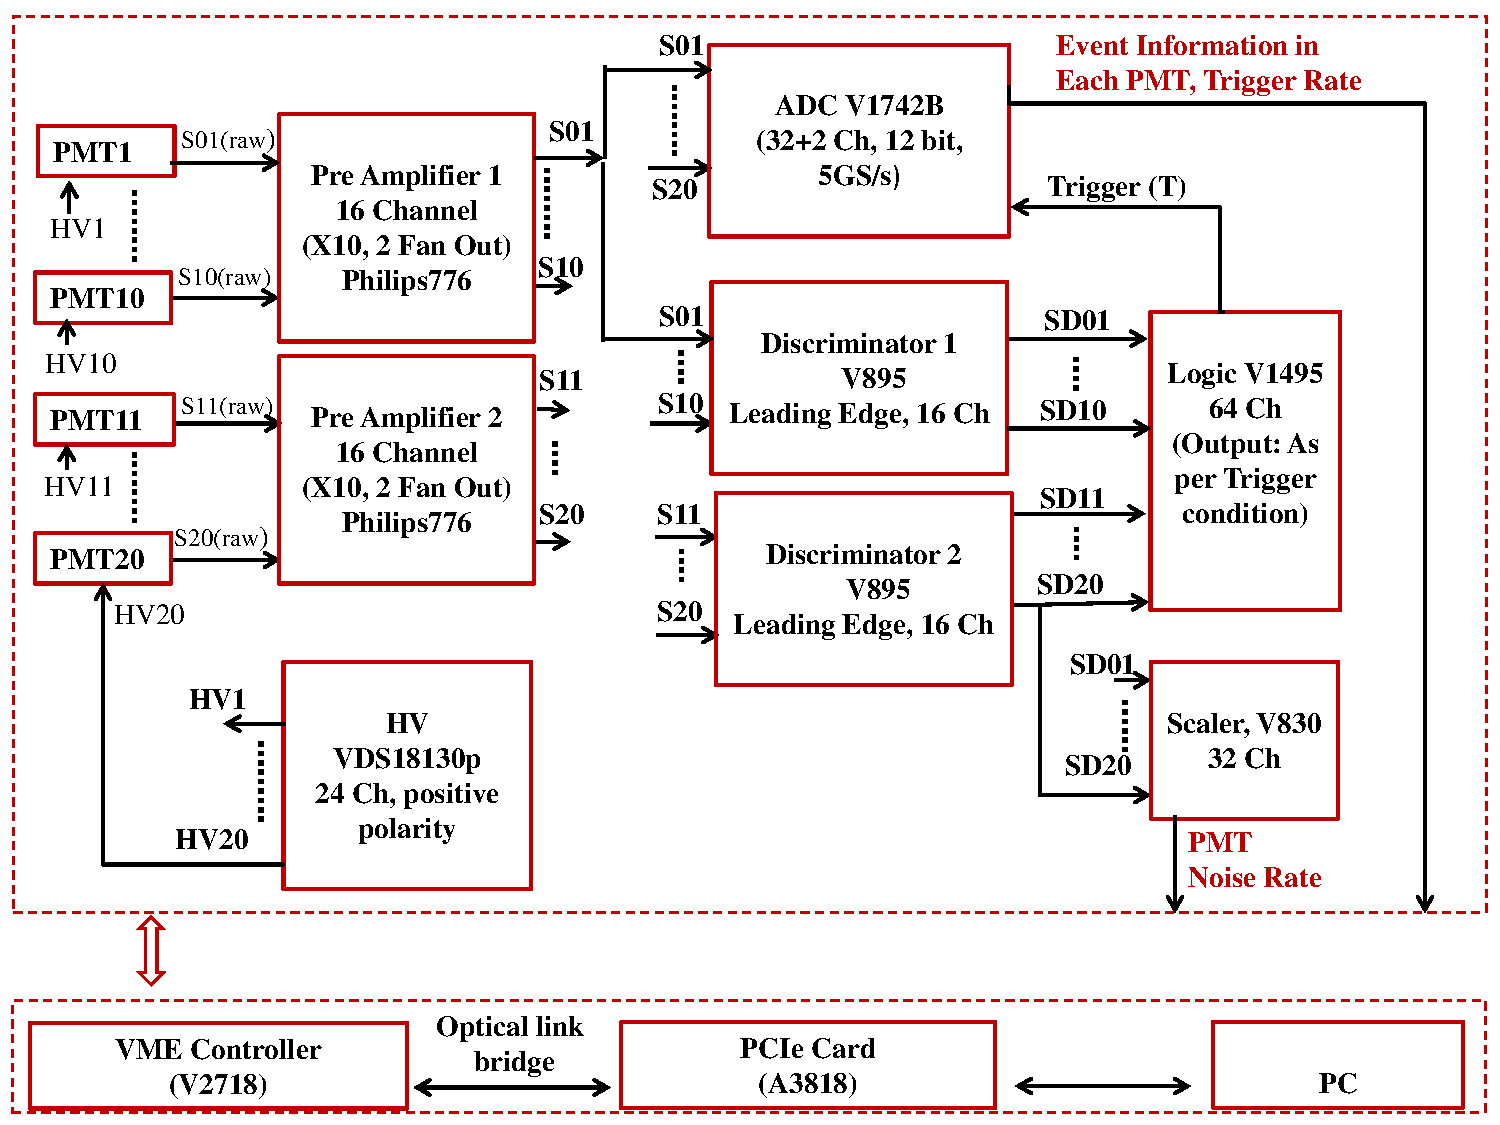
\includegraphics[width=0.85\textwidth]{DAQscheme.pdf}
   \caption{The schematic of the data acquisition system of \direxeno. The 			signal coming from 20 PMTs ({\it i} = 1 -- 20) and the subsequent electronic channels to record the events once triggered. Where S{\it i}(raw) is the raw electrical pulse output of the PMTs, S{\it i} are the amplified pulses, and SD{\it i} are the binary outputs from the discriminator.
}
   \label{Fig:DAQscheme}
\end{figure}
%%%%%%%%%%%%%%%%%%%%%%%%%%%%%%%%%%%%%%%%%%%%%%%%%%%%%%%%%%%%%%%%%%%%%%%%%%%


The ADC consists of two 12\,bit 5\,GS/s switched capacitor digitizer sections, 
each of them with 16+1 channels, based on DRS4 chip. The dynamic range of the input signal is 1\,Vpp with an adjustable DC offset. This module constantly samples (5\,GS/s, 2.5\,GS/s or 2\,GS/s) either bipolar or unipolar analog input 
signals, and records them into circular 
analog memory buffers. Once triggered, all analog memory 
buffers are frozen and digitized into a digital memory buffer 
with a 12 bit resolution. The measured rise time of the system (PMTs, bases, DAQ) is measured to be ($1.4 \pm 0.6$)\,ns, the measured jitter is, $(390 \pm 67)$\,ps. 

The binary output signals from the discriminator are duplicated and fed to 
the logic module\footnote{CAEN V1495: FPGA based general purpose VME board} and to a scaler\footnote{CAEN V830: 16 channel scalar}. 
A global majority trigger is generated in the logic module with the coincidence of any two out of the twenty PMTs within a predefined time window, that will be optimized to reduce dark counts. The event information and trigger rate are read from the ADC, while the individual PMTs trigger rate from the scaler. Further analyses of the relevant events are carried out offline.

\subsection{\textcolor{blue}{The slow control system}}
\label{subsec:sc}


A variety of sensors collect information from the various subsystems, that is being used for monitoring the stability and well-being of the system as well as understanding the complex Xe flow through the system.  
We use a time-series server built specifically for handling events or measurements that are time-stamped based on influxdb~\cite{INFLUXDB}.
For monitoring and visualization we use Grafana~\cite{GRAFANA}, an open source software for time series analytics.
The monitored data is streamed to the database using the influxdb API integrated in python control scripts.

%The copper adapter  holds two $100\Omega$ pt resistor\footnote{PT111 Lakeshore} which are connected to a PID reader\footnote{cryo-con model 18i Cryogenic Temp Monitor} for temperature measurements. 

Ten $100\Omega$ pt resistors\footnote{PT111 Lakeshore}  are installed. Two in the copper adapter attached to the cold finger, and eight around the sphere, pools and pipes. The resistors are connected to a PID reader\footnote{cryo-con model 18i Cryogenic Temp Monitor} for temperature measurements.  To support a readout of more temperature sensors with the same number of feedthroughs data channels we replaced some of the 4-wires PT100 readout channels with a 2-wires one. The temperature-resistance calibration curves were shifted accordingly. The lesser measurment accuracy and stability were more than sufficient to identify liquid-gas transitions and temperature transients.
Pressure/Vacuum reading of the outer- and inner-chamber were done using xxxx and xxxx sensors. 
Termistors based sensors were installed on the cooling water lines, the compressor and near the system for monitoring of the cryocooler operation. They were read using an arduino board with an accuracy of <1 degree.   
The xenon flow rate readings from the MFC are monitored, and a `homemade` switch read by the arduino lets the operator to move between Filling/Recooperation/Circulation modes to allow the proper handling of the flow rate data in the data base (either adding it to the total Xe amount, removing it or no change ).
The PMTs voltage, current and trigger rate are also monitoted and streamed to the database. 

An off-the-shelf USB snake-camera is mounted in the outer vacuum chamber and watching the sphere. The camera si housed in a xx `` nipple with an optical window on one side and a xx bellow on the other opened to the air side. The camera allows the operator to visually inspect the status of the Xe within the sphere. A simple and fast image processing is constantly preformed and the difference between two consecutive optical snapshots is calculated and streamed into the data base.

An additional script is montitoring the database, identifies missing information or other problems based on a set of rules, and alerts the operators via email and sms.




%\clearpage %temporary TBC
